% !TEX program = xelatex
\documentclass[aspectratio=169,professionalfonts]{beamer}

% ============================================================
% Beamer slide deck for the regression assumptions report.
% Math-expanded version for a master's statistics/mathematics class.
% ============================================================

\usetheme{Madrid}
\usecolortheme{seahorse}
\setbeamertemplate{navigation symbols}{}
\setbeamertemplate{caption}[numbered]
\setbeamertemplate{footline}[frame number]

% -- Language and font ---------------------------------------
\usepackage{fontspec}
\usepackage{polyglossia}
\setmainlanguage{vietnamese}
\setotherlanguage{english}
\IfFontExistsTF{Times New Roman}{
  \setmainfont{Times New Roman}
  \setsansfont{Times New Roman}
}{}

% -- Math, graphics, tables ----------------------------------
\usepackage{amsmath, amssymb, mathtools}
\usepackage{graphicx}
\usepackage{booktabs}
\usepackage{tabularx}
\usepackage{array}
\usepackage{xcolor}
\usepackage{listings}

\graphicspath{{figures/}{media/}}

\definecolor{mainblue}{RGB}{0,82,155}
\definecolor{lightblue}{RGB}{235,245,255}
\definecolor{codebg}{RGB}{248,248,248}
\definecolor{codeframe}{RGB}{220,220,220}
\definecolor{codekeyword}{RGB}{0,0,160}
\definecolor{codestring}{RGB}{145,35,35}
\definecolor{codecomment}{RGB}{90,90,90}

\setbeamercolor{title}{fg=mainblue}
\setbeamercolor{frametitle}{fg=mainblue}
\setbeamercolor{block title}{bg=mainblue!10, fg=mainblue}
\setbeamercolor{block body}{bg=lightblue!35, fg=black}

\lstdefinestyle{Rslide}{
  language=R,
  backgroundcolor=\color{codebg},
  frame=single,
  rulecolor=\color{codeframe},
  basicstyle=\ttfamily\scriptsize,
  keywordstyle=\color{codekeyword}\bfseries,
  stringstyle=\color{codestring},
  commentstyle=\color{codecomment}\itshape,
  showstringspaces=false,
  breaklines=true,
  tabsize=2
}

\newcommand{\assumption}[2]{%
  \begin{block}{#1}
    #2
  \end{block}
}

\newcommand{\mathnote}[1]{%
  \begin{block}{Ý nghĩa}
    #1
  \end{block}
}

\title[Các giả định hồi quy bội]{Chủ đề 3: Các Giả Định Quan Trọng\\Của Mô Hình Hồi Quy Bội}
\subtitle{Mô Hình Hóa Thống Kê}
\author[NHÓM 1]{Nguyễn Nhật Quang \and Phạm Đoàn Vịnh Nghi \and Lê Hoàng Như}
\institute[HCMUS]{Trường Đại học Khoa học Tự Nhiên - ĐHQGHCM\\Giảng viên: TS. Nguyễn Thị Mộng Ngọc}
\date{}

\hypersetup{
  pdftitle={Beamer - Các Giả Định Quan Trọng Của Mô Hình Hồi Quy Bội},
  pdfauthor={Nguyễn Nhật Quang, Phạm Đoàn Vịnh Nghi, Lê Hoàng Như}
}


% -- Section divider -----------------------------------------
\AtBeginSection[]{
  \begin{frame}[plain]
    \vfill
    \begin{flushleft}
      {\Large\bfseries\color{mainblue} Phần \insertsectionnumber}\\[0.35cm]
      {\Huge\bfseries\color{mainblue} \insertsection}\\[0.25cm]
      {\rule{0.68\textwidth}{1.2pt}}
    \end{flushleft}
    \vfill
  \end{frame}
}

\begin{document}

% 1
\begin{frame}
  \titlepage
  \vspace{-0.2cm}
  \begin{center}
    {\small Nhóm thực hiện: NHÓM 1}
  \end{center}
\end{frame}

% 2
\begin{frame}{Nhóm Thực Hiện}
  \small
  \begin{tabularx}{\textwidth}{@{}lclX@{}}
    \toprule
    \textbf{Thành viên} & \textbf{Mã học viên} & & \textbf{Nhiệm vụ chính} \\
    \midrule
    Nguyễn Nhật Quang & 25C23002 && Tính tuyến tính; tính chuẩn; tổng hợp báo cáo; thuyết trình \\
    Phạm Đoàn Vịnh Nghi & 25C23012 && Tính độc lập; phân công nhiệm vụ; câu hỏi thảo luận; thuyết trình \\
    Lê Hoàng Như & 25C23014 && Đồng nhất phương sai; dàn ý; tổng hợp, kết luận; thuyết trình \\
    \bottomrule
  \end{tabularx}
\end{frame}

% 3
\begin{frame}{Agenda}
  \begin{columns}[T,onlytextwidth]
    \column{0.48\textwidth}
      \begin{enumerate}
        \item Tổng quan hồi quy bội
        \item Giả định tuyến tính
        \item Giả định chuẩn của sai số
      \end{enumerate}
    \column{0.48\textwidth}
      \begin{enumerate}
        \setcounter{enumi}{3}
        \item Đồng nhất phương sai
        \item Tính độc lập của sai số
        \item Workflow kiểm tra giả định
      \end{enumerate}
  \end{columns}
  \vspace{0.45cm}
  \assumption{Câu hỏi trung tâm}{Giả định nào bảo vệ hệ số OLS, giả định nào bảo vệ sai số chuẩn, và giả định nào bảo vệ phân phối kiểm định?}
\end{frame}

% 4
\begin{frame}{Bản Đồ Giả Định Trong Hồi Quy Bội}
  \small
  \begin{tabularx}{\textwidth}{@{}>{\bfseries}l>{\raggedright\arraybackslash}X>{\raggedright\arraybackslash}X@{}}
    \toprule
    Giả định & Điều kiện toán học & Bảo vệ điều gì? \\
    \midrule
    Tuyến tính & $E(Y\mid X)$ đúng dạng theo tham số & Hệ số và diễn giải quan hệ trung bình \\
    Chuẩn & $\varepsilon\mid X\sim N(0,\sigma^2I)$ & Suy diễn mẫu nhỏ: $t$, $F$, $\chi^2$ \\
    Đồng nhất phương sai & $\mathrm{Var}(\varepsilon_i\mid X)=\sigma^2$ & Công thức SE cổ điển \\
    Tính độc lập của sai số & $\varepsilon_i\perp\!\!\!\perp\varepsilon_j\mid X$; thường kiểm tra qua $\mathrm{Cov}_{ij}=0$ & SE, kiểm định và khoảng tin cậy khi dữ liệu có thứ tự \\
    \bottomrule
  \end{tabularx}
\end{frame}

% 5
\section{Tổng Quan: Hồi Quy Bội}
\begin{frame}{Hồi Quy Là Gì?}
  \small
  Hồi quy là phương pháp thống kê dùng để mô tả, định lượng và dự báo mối quan hệ giữa biến phản ứng $Y$ và một hoặc nhiều biến dự báo $X$.
  \[
    \text{Trọng tâm của hồi quy:}\qquad E(Y\mid X).
  \]
  \begin{block}{Cách hiểu}
    Với mỗi mức giá trị của $X$, hồi quy hỏi: giá trị trung bình của $Y$ thay đổi như thế nào?
  \end{block}
  \begin{itemize}
    \item Dùng để giải thích: biến nào liên quan đến $Y$?
    \item Dùng để dự báo: $Y$ kỳ vọng là bao nhiêu khi biết $X$?
    \item Dùng để suy diễn: tác động ước lượng có đáng tin không?
  \end{itemize}
\end{frame}

% 6
\begin{frame}{Mô Hình Hồi Quy Là Gì?}
  \small
  Một mô hình hồi quy tách $Y$ thành hai phần:
  \[
    Y_i = m(x_i)+\varepsilon_i,
    \qquad
    E(\varepsilon_i\mid x_i)=0.
  \]
  \begin{tabularx}{\textwidth}{@{}lX@{}}
    \toprule
    Thành phần & Ý nghĩa \\
    \midrule
    $m(x_i)=E(Y_i\mid x_i)$ & phần có cấu trúc, hay quan hệ trung bình có điều kiện \\
    $\varepsilon_i$ & phần sai số ngẫu nhiên quanh quan hệ trung bình \\
    \bottomrule
  \end{tabularx}
  \vspace{0.25cm}
  \mathnote{Các giả định hồi quy chủ yếu nói về dạng của $m(x)$ và cấu trúc của sai số $\varepsilon$.}
\end{frame}

% 7
\begin{frame}{OLS Là Gì và BLUE Là Gì?}
  \footnotesize
  \begin{columns}[T,onlytextwidth]
    \column{0.48\textwidth}
      \begin{block}{OLS}
        Chọn hệ số để tối thiểu hóa tổng bình phương phần dư:
        \[
          \hat{\boldsymbol{\beta}}_{OLS}
          =
          \arg\min_{\boldsymbol{\beta}}
          \sum_{i=1}^{n}(y_i-\hat y_i)^2.
        \]
        Khi $\mathbf{X}^{\top}\mathbf{X}$ khả nghịch:
        \[
          \hat{\boldsymbol{\beta}}_{OLS}
          =
          (\mathbf{X}^{\top}\mathbf{X})^{-1}
          \mathbf{X}^{\top}\mathbf{y}.
        \]
      \end{block}
    \column{0.48\textwidth}
      \begin{block}{BLUE}
        Theo Gauss--Markov, với mọi ước lượng tuyến tính không chệch $\tilde{\boldsymbol{\beta}}$:
        \[
          \mathrm{Var}(\tilde{\boldsymbol{\beta}}\mid \mathbf{X})
          -
          \mathrm{Var}(\hat{\boldsymbol{\beta}}_{OLS}\mid \mathbf{X})
          \succeq 0.
        \]
        Nghĩa là OLS có phương sai nhỏ nhất trong lớp tuyến tính không chệch.
      \end{block}
  \end{columns}
\end{frame}

% 8
\begin{frame}{Mô Hình Hồi Quy Bội Là Gì?}
  \small
  Hồi quy tuyến tính đơn dùng một biến dự báo:
  \[
    Y_i=\beta_0+\beta_1X_i+\varepsilon_i.
  \]
  Hồi quy bội mở rộng sang nhiều biến dự báo:
  \[
    Y_i=\beta_0+\beta_1X_{i1}+\beta_2X_{i2}+\cdots+\beta_kX_{ik}+\varepsilon_i.
  \]
  \begin{block}{Ý nghĩa hệ số}
    $\beta_j$ là thay đổi trung bình của $Y$ khi $X_j$ tăng một đơn vị, trong khi giữ các biến dự báo còn lại không đổi.
  \end{block}
\end{frame}

% 9
\begin{frame}{Mô Hình Hồi Quy Bội Dạng Ma Trận}
  \small
  \[
    \mathbf{y}=\mathbf{X}\boldsymbol{\beta}+\boldsymbol{\varepsilon},
    \qquad
    E(\boldsymbol{\varepsilon}\mid \mathbf{X})=\mathbf{0}.
  \]
  \vspace{-0.1cm}
  \begin{tabularx}{\textwidth}{@{}lX@{}}
    \toprule
    Ký hiệu & Diễn giải \\
    \midrule
    $\mathbf{y}\in\mathbb{R}^{n}$ & vector biến phản hồi \\
    $\mathbf{X}\in\mathbb{R}^{n\times k}$ & ma trận thiết kế, gồm các biến dự báo \\
    $\boldsymbol{\beta}\in\mathbb{R}^{k}$ & vector tham số cần ước lượng \\
    $\boldsymbol{\varepsilon}\in\mathbb{R}^{n}$ & sai số ngẫu nhiên, phần không giải thích bởi quan hệ trung bình \\
    \bottomrule
  \end{tabularx}
\end{frame}

% 10
\begin{frame}{OLS Là Một Bài Toán Tối Ưu}
  \small
  OLS chọn hệ số làm nhỏ nhất tổng bình phương phần dư:
  \[
    \hat{\boldsymbol{\beta}}
    =
    \arg\min_{\boldsymbol{\beta}}
    (\mathbf{y}-\mathbf{X}\boldsymbol{\beta})^{\top}
    (\mathbf{y}-\mathbf{X}\boldsymbol{\beta}).
  \]
  Đạo hàm theo $\boldsymbol{\beta}$:
  \[
    \frac{\partial}{\partial\boldsymbol{\beta}}
    \|\mathbf{y}-\mathbf{X}\boldsymbol{\beta}\|^2
    =
    -2\mathbf{X}^{\top}(\mathbf{y}-\mathbf{X}\boldsymbol{\beta}).
  \]
  \mathnote{OLS là nghiệm của một bài toán hình học: chiếu $\mathbf{y}$ lên không gian cột của $\mathbf{X}$.}
\end{frame}

% 11
\begin{frame}{Normal Equations và Nghiệm Đóng}
  \small
  Điều kiện bậc nhất tạo ra normal equations:
  \[
    \mathbf{X}^{\top}(\mathbf{y}-\mathbf{X}\hat{\boldsymbol{\beta}})=\mathbf{0}
    \quad\Longleftrightarrow\quad
    \mathbf{X}^{\top}\mathbf{X}\hat{\boldsymbol{\beta}}=\mathbf{X}^{\top}\mathbf{y}.
  \]
  Nếu $\mathbf{X}^{\top}\mathbf{X}$ khả nghịch:
  \[
    \hat{\boldsymbol{\beta}}
    =
    (\mathbf{X}^{\top}\mathbf{X})^{-1}\mathbf{X}^{\top}\mathbf{y}.
  \]
  \begin{block}{Điểm kiểm tra}
    Công thức này tồn tại do cấu trúc tuyến tính theo tham số, không do giả định normality.
  \end{block}
\end{frame}

% 12
\begin{frame}{Hat Matrix: Dự Báo Là Phép Chiếu}
  \small
  \[
    \hat{\mathbf{y}}=\mathbf{X}\hat{\boldsymbol{\beta}}
    =\mathbf{X}(\mathbf{X}^{\top}\mathbf{X})^{-1}\mathbf{X}^{\top}\mathbf{y}
    =\mathbf{H}\mathbf{y}.
  \]
  \[
    \mathbf{H}=\mathbf{X}(\mathbf{X}^{\top}\mathbf{X})^{-1}\mathbf{X}^{\top},
    \qquad
    \mathbf{e}=\mathbf{y}-\hat{\mathbf{y}}=(\mathbf{I}-\mathbf{H})\mathbf{y}.
  \]
  \begin{columns}[T,onlytextwidth]
    \column{0.48\textwidth}
      \assumption{Tính chất}{$\mathbf{H}^2=\mathbf{H}$, $\mathbf{H}^{\top}=\mathbf{H}$; $\mathbf{X}^{\top}\mathbf{e}=0$.}
    \column{0.48\textwidth}
      \assumption{Leverage}{$h_{ii}$ đo mức ảnh hưởng hình học của quan sát $i$ lên giá trị khớp.}
  \end{columns}
\end{frame}

% 13
\begin{frame}{Mỗi Giả Định Đụng Vào Một Ma Trận Khác Nhau}
  \small
  \[
    \hat{\boldsymbol{\beta}}-\boldsymbol{\beta}
    =
    (\mathbf{X}^{\top}\mathbf{X})^{-1}\mathbf{X}^{\top}\boldsymbol{\varepsilon}.
  \]
  \begin{tabularx}{\textwidth}{@{}lX@{}}
    \toprule
    Nếu muốn kết luận... & Cần kiểm soát... \\
    \midrule
    $\hat{\boldsymbol{\beta}}$ không chệch & $E(\boldsymbol{\varepsilon}\mid\mathbf{X})=0$ \\
    SE cổ điển đúng & $\mathrm{Var}(\boldsymbol{\varepsilon}\mid\mathbf{X})=\sigma^2\mathbf{I}$ \\
    Suy diễn mẫu nhỏ chính xác & $\boldsymbol{\varepsilon}\mid\mathbf{X}\sim N(0,\sigma^2\mathbf{I})$ \\
    Dữ liệu có thứ tự không làm sai SE & Không có phần tử ngoài đường chéo trong covariance \\
    \bottomrule
  \end{tabularx}
\end{frame}

% 14
\begin{frame}{Bốn Rủi Ro Thống Kê Chính}
  \small
  \begin{enumerate}
    \item Sai dạng $E(Y\mid X)$ $\Rightarrow$ hệ số có thể bị chệch.
    \item Không chuẩn $\Rightarrow$ phân phối $t/F/\chi^2$ mẫu nhỏ mất cơ sở chính xác.
    \item Phương sai thay đổi $\Rightarrow$ SE cổ điển dùng sai ma trận hiệp phương sai.
    \item Tự tương quan $\Rightarrow$ covariance có phần tử ngoài đường chéo, SE cổ điển sai.
  \end{enumerate}
  \vspace{0.25cm}
  \assumption{Logic của bài}{Không kiểm tra giả định để ``làm đẹp'' mô hình; kiểm tra để biết kết luận nào còn đáng tin.}
\end{frame}

% 15
\section{Tuyến Tính}
\begin{frame}{Tuyến Tính: Theo Tham Số, Không Nhất Thiết Theo Biến}
  \small
  \begin{columns}[T,onlytextwidth]
    \column{0.53\textwidth}
      \[
        E(Y\mid X)=\beta_0+\beta_1X+\beta_2X^2
      \]
      Tuyến tính theo $\boldsymbol{\beta}$ dù có $X^2$.
      \[
        E(Y\mid X)=\beta_0+\beta_1\log(X)
      \]
      Tuyến tính theo $\boldsymbol{\beta}$ dù biến đã biến đổi.
    \column{0.43\textwidth}
      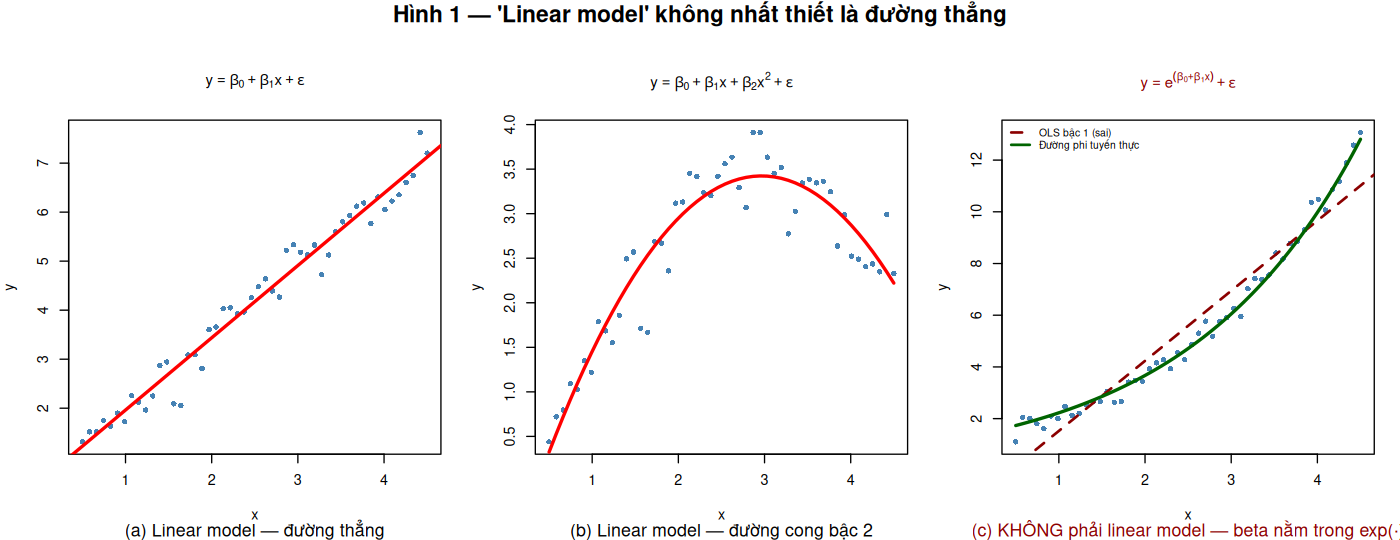
\includegraphics[width=\textwidth]{fig1_linear_params.png}
  \end{columns}
\end{frame}

% 16
\begin{frame}{Cần Chọn Đúng Dạng Cho \texorpdfstring{$E(Y\mid X)$}{E(Y|X)}}
  \small
  \[
    E(Y\mid X)=m(X),
    \qquad
    \text{mô hình OLS giả sử } m(X)=X\beta.
  \]
  Nếu $m(X)$ thật không nằm trong không gian mô hình đã chọn, ta có:
  \[
    Y=X\beta + r(X)+\varepsilon,
  \]
  với $r(X)$ là phần sai đặc tả. Khi đó điều kiện then chốt trở thành:
  \[
    E(r(X)+\varepsilon\mid X)\neq 0.
  \]
  \mathnote{Vi phạm tuyến tính thường nguy hiểm hơn heteroscedasticity vì nó có thể làm hỏng chính hệ số.}
\end{frame}

% 17
\begin{frame}{Điều Kiện Ngoại Sinh và Không Chệch}
  \small
  Từ công thức sai lệch:
  \[
    \hat{\boldsymbol{\beta}}-\boldsymbol{\beta}
    =
    (\mathbf{X}^{\top}\mathbf{X})^{-1}\mathbf{X}^{\top}\boldsymbol{\varepsilon}.
  \]
  Lấy kỳ vọng có điều kiện theo $\mathbf{X}$:
  \[
    E(\hat{\boldsymbol{\beta}}-\boldsymbol{\beta}\mid\mathbf{X})
    =
    (\mathbf{X}^{\top}\mathbf{X})^{-1}\mathbf{X}^{\top}
    E(\boldsymbol{\varepsilon}\mid\mathbf{X}).
  \]
  \begin{block}{Kết luận}
    Nếu $E(\boldsymbol{\varepsilon}\mid\mathbf{X})=0$, OLS không chệch. Nếu $E(Y\mid X)$ bị chọn sai dạng, điều kiện này thường thất bại.
  \end{block}
\end{frame}

% 18
\begin{frame}{Gauss-Markov: BLUE Không Cần Normality}
  \small
  Dưới các điều kiện chính:
  \begin{itemize}
    \item $E(\boldsymbol{\varepsilon}\mid\mathbf{X})=0$,
    \item $\mathrm{Var}(\boldsymbol{\varepsilon}\mid\mathbf{X})=\sigma^2\mathbf{I}$,
    \item $\mathbf{X}^{\top}\mathbf{X}$ khả nghịch,
  \end{itemize}
  OLS là \textbf{Best Linear Unbiased Estimator}:
  \[
    \mathrm{Var}(\tilde{\boldsymbol{\beta}}\mid X)
    -
    \mathrm{Var}(\hat{\boldsymbol{\beta}}\mid X)
    \succeq 0
  \]
  với mọi ước lượng tuyến tính không chệch $\tilde{\boldsymbol{\beta}}$.
\end{frame}

% 19
\begin{frame}{Hình Học Projection Của OLS}
  \small
  \begin{columns}[T,onlytextwidth]
    \column{0.46\textwidth}
      \[
        \hat{\mathbf{y}}=\mathbf{H}\mathbf{y},
        \qquad
        \mathbf{e}=(\mathbf{I}-\mathbf{H})\mathbf{y}.
      \]
      \[
        \mathbf{X}^{\top}\mathbf{e}=0.
      \]
      Nghĩa là phần dư vuông góc với mọi cột của $\mathbf{X}$.
    \column{0.50\textwidth}
      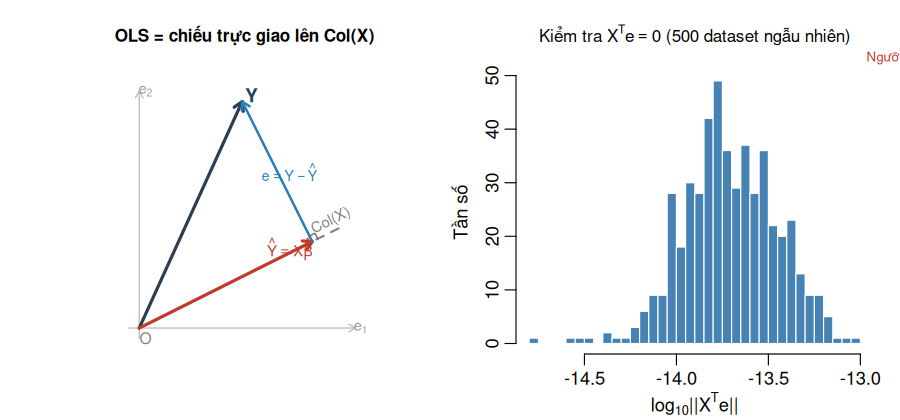
\includegraphics[width=\textwidth,height=0.65\textheight,keepaspectratio]{fig10_projection.png}
  \end{columns}
\end{frame}

% 20
\begin{frame}{Khi Tuyến Tính Sai: Bias Không Biến Mất Bằng Robust SE}
  \small
  Nếu mô hình thật là:
  \[
    \mathbf{y}=\mathbf{X}\boldsymbol{\beta}+\mathbf{g}+\boldsymbol{\varepsilon},
  \]
  nhưng ta fit mô hình thiếu $\mathbf{g}$, thì:
  \[
    E(\hat{\boldsymbol{\beta}}\mid X)
    =
    \boldsymbol{\beta}
    +
    (\mathbf{X}^{\top}\mathbf{X})^{-1}\mathbf{X}^{\top}\mathbf{g}.
  \]
  \assumption{Thông điệp}{Sai số chuẩn vững chỉ sửa covariance của hệ số; nó không sửa bias do $E(Y\mid X)$ bị chọn sai dạng.}
\end{frame}

% 21
\begin{frame}{Dữ Liệu Có Thể Đánh Lừa: Anscombe}
  \begin{columns}[T,onlytextwidth]
    \column{0.38\textwidth}
      \small
      \begin{itemize}
        \item Cùng mean, variance, correlation và regression line.
        \item Quan hệ thật lại rất khác nhau.
        \item Summary statistics không thay thế đồ thị.
      \end{itemize}
    \column{0.58\textwidth}
      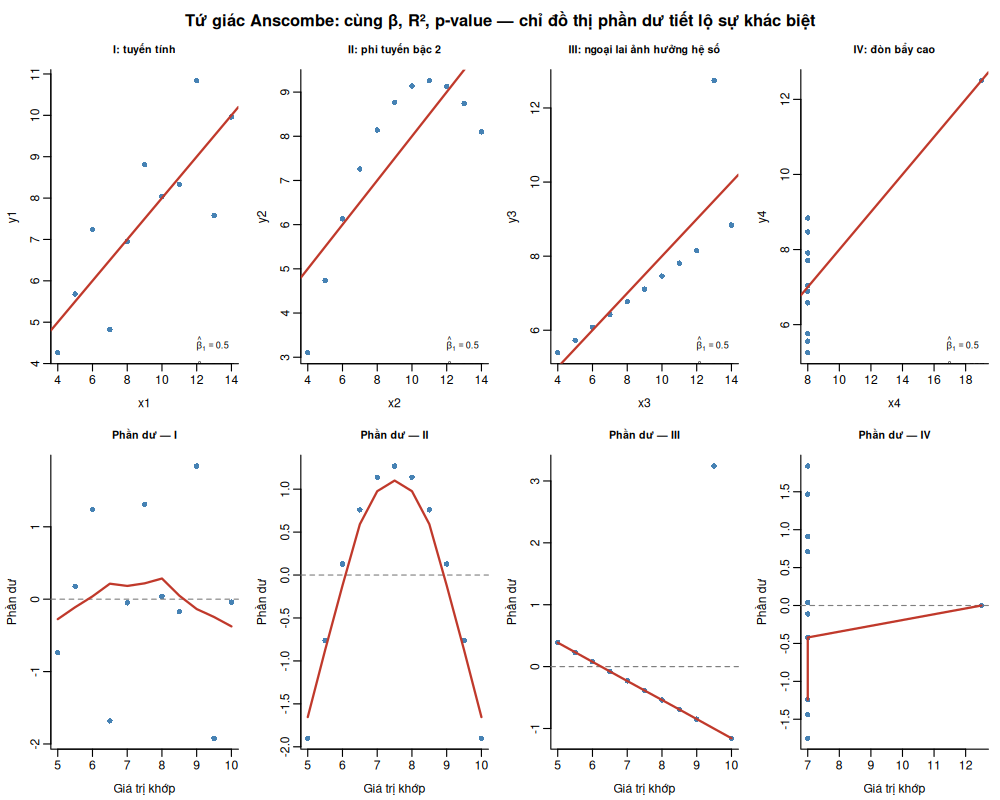
\includegraphics[width=\textwidth,height=0.68\textheight,keepaspectratio]{fig7_anscombe.png}
  \end{columns}
\end{frame}

% 22
\begin{frame}{Residual Plot: Kiểm Tra Quan Hệ Trung Bình}
  \begin{columns}[T,onlytextwidth]
    \column{0.38\textwidth}
      \small
      \begin{itemize}
        \item Nếu $E(Y\mid X)$ được mô tả hợp lý, phần dư không nên còn pattern hệ thống.
        \item Dạng cong gợi ý thiếu biến đổi, bậc hai, tương tác hoặc spline.
      \end{itemize}
      \assumption{Dấu hiệu cảnh báo}{Phần dư có xu hướng cong, cụm hoặc thay đổi có hệ thống theo fitted values.}
    \column{0.58\textwidth}
      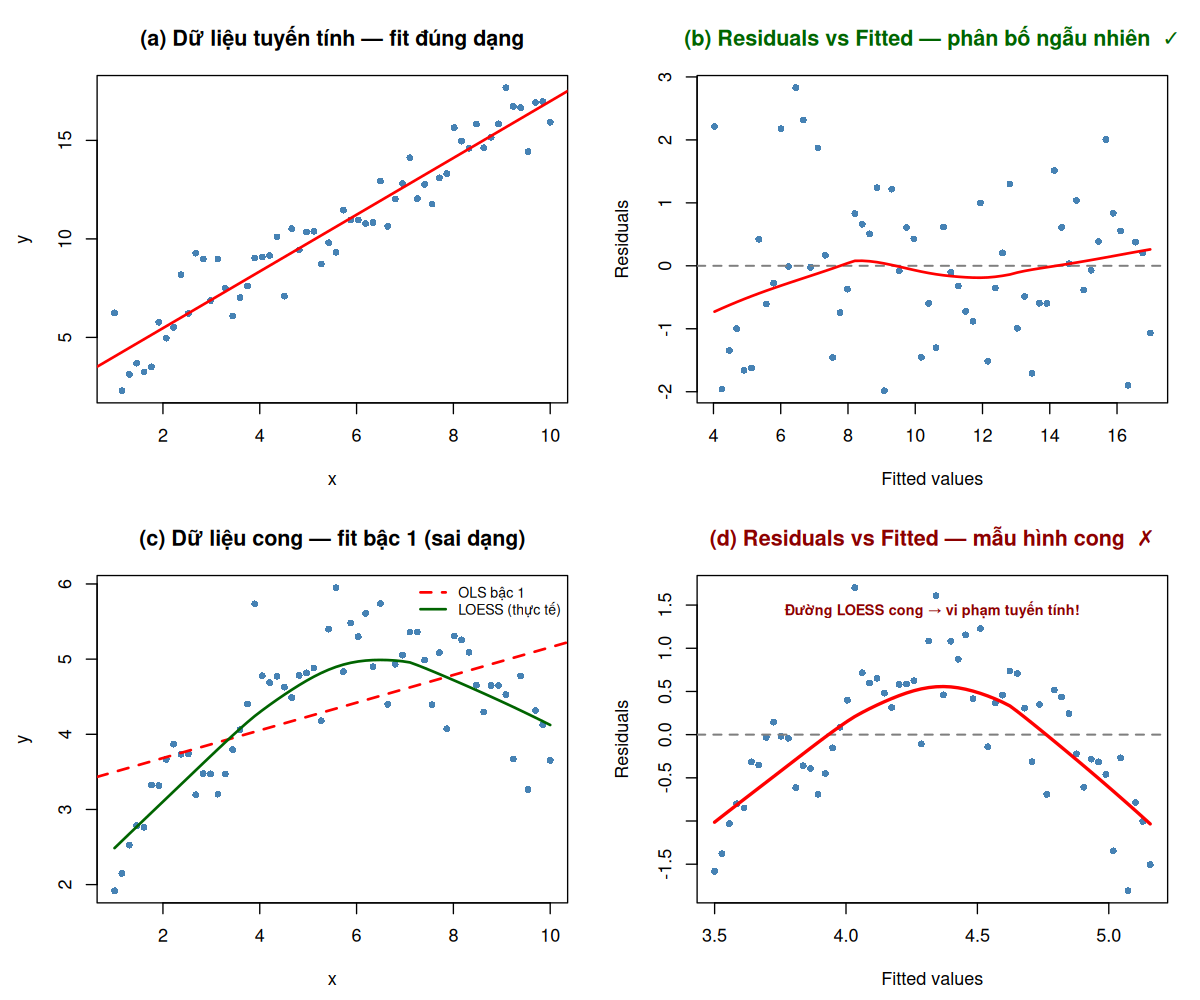
\includegraphics[width=\textwidth,height=0.68\textheight,keepaspectratio]{fig3_residual_plots.png}
  \end{columns}
\end{frame}

% 23
\begin{frame}{Công Cụ Chẩn Đoán Tuyến Tính}
  \small
  \begin{tabularx}{\textwidth}{@{}l>{\raggedright\arraybackslash}X>{\raggedright\arraybackslash}X@{}}
    \toprule
    Công cụ & Đọc điều gì? & Rủi ro phát hiện \\
    \midrule
    Scatterplot matrix & Quan hệ thô giữa các biến & Phi tuyến rõ, outlier \\
    Residuals vs fitted & Pattern còn sót trong phần dư & Sai dạng $E(Y\mid X)$ \\
    Added-variable plot & Đóng góp của từng biến sau khi đã kiểm soát biến khác & Biến thiếu, phi tuyến theo biến riêng \\
    Tukey nonadditivity & Dấu hiệu không cộng tính & Thiếu tương tác/biến đổi \\
    \bottomrule
  \end{tabularx}
\end{frame}

% 24
\begin{frame}{Khắc Phục Phi Tuyến: Vẫn Có Thể Giữ Tư Duy Tuyến Tính}
  \small
  \begin{tabularx}{\textwidth}{@{}lXX@{}}
    \toprule
    Cách xử lý & Dạng mô hình & Khi dùng \\
    \midrule
    Biến đổi biến & $Y\sim \log X$ hoặc $\log Y\sim X$ & Quan hệ cong đơn giản \\
    Đa thức & $Y\sim X+X^2+\cdots$ & Có độ cong hoặc cực trị \\
    Splines & $Y\sim B_1(X)+\cdots+B_m(X)$ & Quan hệ phi tuyến mềm \\
    GLM & $g(EY)=X\beta$ & Dữ liệu count, binary, rate \\
    \bottomrule
  \end{tabularx}
  \vspace{0.15cm}
  \begin{center}
    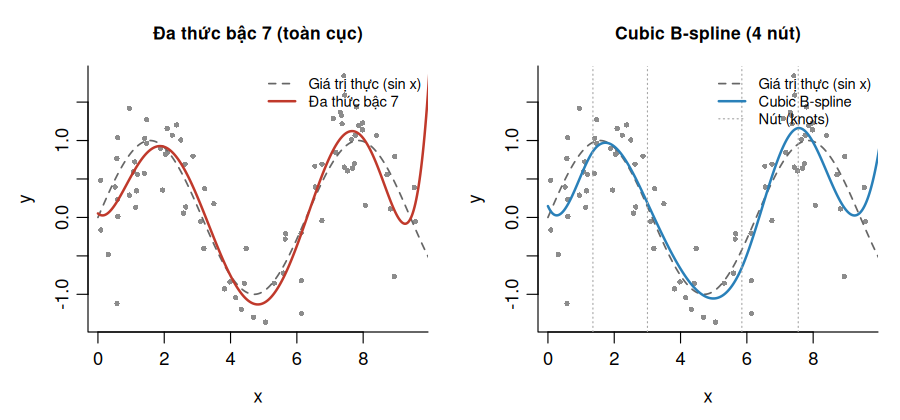
\includegraphics[width=0.50\textwidth,height=0.34\textheight,keepaspectratio]{fig9_splines.png}
  \end{center}
\end{frame}

% 25
\begin{frame}{Kết Quả Nâng Cao: Li-Duan}
  \small
  Một kết quả trong report: nếu mô hình thật có dạng single-index ẩn
  \[
    Y=g(\boldsymbol{\beta}^{\top}X)+\varepsilon,
  \]
  và $X$ có phân phối đối xứng elip, OLS vẫn phục hồi đúng hướng:
  \[
    \hat{\boldsymbol{\beta}}_{OLS}\xrightarrow{p} c\boldsymbol{\beta},
    \qquad c\neq 0.
  \]
  \begin{columns}[T,onlytextwidth]
    \column{0.45\textwidth}
      \mathnote{Dấu và thứ tự quan trọng tương đối có thể được bảo toàn, dù độ lớn bị scale.}
    \column{0.50\textwidth}
      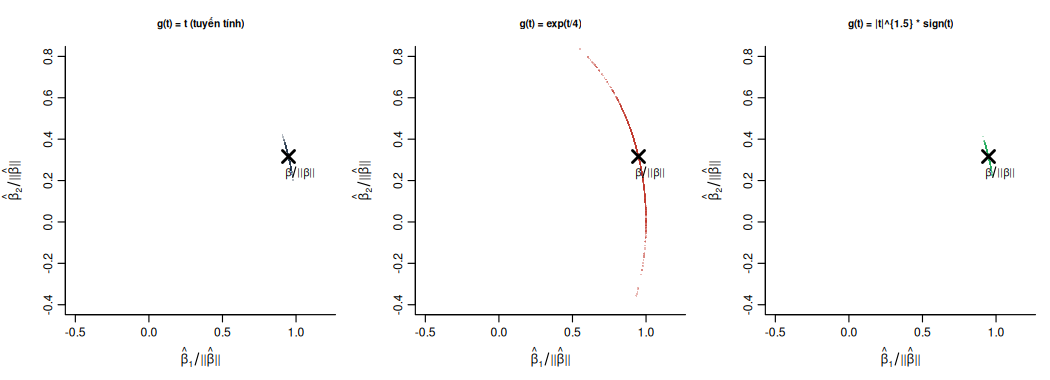
\includegraphics[width=\textwidth,height=0.40\textheight,keepaspectratio]{fig11_liduan.png}
  \end{columns}
\end{frame}

% 26
\section{Tính Chuẩn}
\begin{frame}{Giả Định Chuẩn Là Gì?}
  \small
  Giả định mẫu nhỏ cổ điển thường viết:
  \[
    \boldsymbol{\varepsilon}\mid\mathbf{X}\sim
    N(\mathbf{0},\sigma^2\mathbf{I}).
  \]
  Khi đó:
  \[
    \mathbf{Y}\mid\mathbf{X}
    \sim
    N(\mathbf{X}\boldsymbol{\beta},\sigma^2\mathbf{I}).
  \]
  \assumption{Điểm dễ nhầm}{Ta không yêu cầu $Y$ chuẩn biên; điều kiện là phân phối sai số quanh hàm kỳ vọng có điều kiện.}
\end{frame}

% 27
\begin{frame}{Phân Phối Của \texorpdfstring{$\hat\beta$}{beta-hat} Khi Sai Số Chuẩn}
  \small
  Vì $\hat{\boldsymbol{\beta}}$ là biến đổi tuyến tính của $\mathbf{Y}$:
  \[
    \hat{\boldsymbol{\beta}}
    =
    (\mathbf{X}^{\top}\mathbf{X})^{-1}\mathbf{X}^{\top}\mathbf{Y},
  \]
  nếu $\mathbf{Y}\mid X$ chuẩn thì:
  \[
    \hat{\boldsymbol{\beta}}\mid X
    \sim
    N\left(
      \boldsymbol{\beta},
      \sigma^2(\mathbf{X}^{\top}\mathbf{X})^{-1}
    \right).
  \]
  \mathnote{Đây là cơ sở trực tiếp cho kiểm định hệ số trong mẫu nhỏ.}
\end{frame}

% 28
\begin{frame}{Ước Lượng \texorpdfstring{$\sigma^2$}{sigma2} và Phân Phối \texorpdfstring{$\chi^2$}{chi-square}}
  \small
  \[
    s^2=\frac{\mathbf{e}^{\top}\mathbf{e}}{n-k}
    =\frac{SSE}{n-k}.
  \]
  Nếu $\varepsilon\mid X\sim N(0,\sigma^2I)$:
  \[
    \frac{(n-k)s^2}{\sigma^2}
    =
    \frac{\mathbf{e}^{\top}\mathbf{e}}{\sigma^2}
    \sim
    \chi^2_{n-k}.
  \]
  \begin{block}{Ý nghĩa}
    Normality giúp suy diễn về phương sai và các thống kê $t/F$ có phân phối chính xác.
  \end{block}
\end{frame}

% 29
\begin{frame}{Kiểm Định \texorpdfstring{$t$}{t} Cho Một Hệ Số}
  \small
  Với hệ số thứ $j$:
  \[
    SE(\hat\beta_j)=s\sqrt{[(\mathbf{X}^{\top}\mathbf{X})^{-1}]_{jj}}.
  \]
  Kiểm định $H_0:\beta_j=\beta_{j,0}$ dùng:
  \[
    t_j
    =
    \frac{\hat\beta_j-\beta_{j,0}}{SE(\hat\beta_j)}
    \sim t_{n-k}
    \quad \text{dưới }H_0.
  \]
  \mathnote{Nếu normality không đúng và mẫu nhỏ, phân phối $t$ chính xác này không còn được đảm bảo.}
\end{frame}

% 30
\begin{frame}{Kiểm Định \texorpdfstring{$F$}{F} Cho Ràng Buộc Tuyến Tính}
  \small
  Với $q$ ràng buộc tuyến tính $H_0: R\beta=r$:
  \[
    F
    =
    \frac{(R\hat\beta-r)^{\top}
    [R(\mathbf{X}^{\top}\mathbf{X})^{-1}R^{\top}]^{-1}
    (R\hat\beta-r)/q}{s^2}
    \sim F_{q,n-k}.
  \]
  \begin{block}{Vai trò}
    $F$-test tổng thể và partial $F$-test dựa trên cùng nền tảng normality + homoscedasticity + independence.
  \end{block}
\end{frame}

% 31
\begin{frame}{Phần Dư Không Phải Sai Số Thật}
  \small
  \[
    \mathbf{e}=(\mathbf{I}-\mathbf{H})\mathbf{Y}
    =
    (\mathbf{I}-\mathbf{H})\boldsymbol{\varepsilon}.
  \]
  Do đó:
  \[
    E(\mathbf{e}\mid X)=0,
    \qquad
    \mathrm{Var}(\mathbf{e}\mid X)=\sigma^2(\mathbf{I}-\mathbf{H}).
  \]
  Với từng quan sát:
  \[
    \mathrm{Var}(e_i\mid X)=\sigma^2(1-h_{ii}).
  \]
  \assumption{Hệ quả}{Residuals có variance khác nhau ngay cả khi sai số thật đồng nhất phương sai.}
\end{frame}

% 32
\begin{frame}{Q-Q Plot và Dạng Lệch Phân Phối}
  \begin{columns}[T,onlytextwidth]
    \column{0.38\textwidth}
      \small
      \begin{itemize}
        \item Lệch ở giữa: dạng $E(Y\mid X)$ có thể sai.
        \item Lệch ở đuôi: outlier hoặc đuôi nặng.
        \item Một vài điểm cực đoan cần xem leverage/Cook's distance.
      \end{itemize}
    \column{0.58\textwidth}
      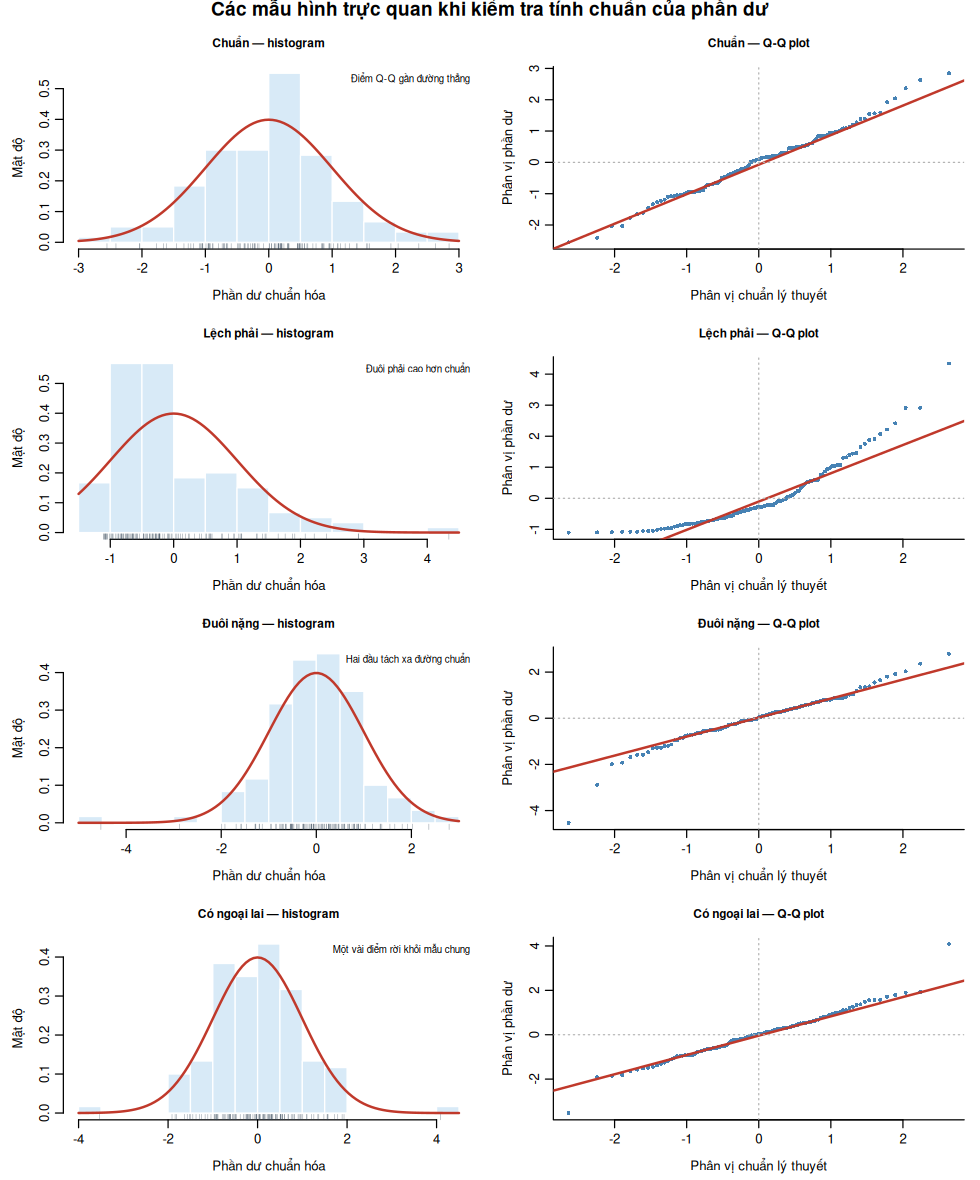
\includegraphics[width=\textwidth,height=0.68\textheight,keepaspectratio]{fig16_normality_patterns.png}
  \end{columns}
\end{frame}

% 33
\begin{frame}{Shapiro-Wilk: Ý Tưởng Kiểm Định}
  \small
  Shapiro-Wilk so sánh ordered residuals với ordered statistics kỳ vọng từ chuẩn:
  \[
    W
    =
    \frac{\left(\sum_{i=1}^{n} a_i e_{(i)}\right)^2}
    {\sum_{i=1}^{n}(e_i-\bar e)^2}.
  \]
  \begin{itemize}
    \item $e_{(i)}$ là phần dư đã sắp xếp.
    \item Hệ số $a_i$ đến từ phân phối chuẩn thứ tự.
    \item Nhạy trong mẫu nhỏ/vừa, nhưng p-value cần đọc cùng Q-Q plot.
  \end{itemize}
\end{frame}

% 34
\begin{frame}{Jarque-Bera: Skewness và Kurtosis}
  \small
  Jarque-Bera kiểm tra hai moment bậc cao:
  \[
    JB
    =
    \frac{n}{6}
    \left(
      S^2+\frac{(K-3)^2}{4}
    \right)
    \sim \chi^2_2.
  \]
  \begin{tabularx}{\textwidth}{@{}lX@{}}
    \toprule
    Thành phần & Ý nghĩa \\
    \midrule
    $S$ & skewness, đo lệch đối xứng \\
    $K$ & kurtosis, đo độ dày đuôi so với chuẩn \\
    $K-3$ & excess kurtosis, bằng 0 nếu chuẩn \\
    \bottomrule
  \end{tabularx}
\end{frame}

% 35
\begin{frame}{Mẫu Lớn: CLT Giúp Nhưng Không Cứu Tất Cả}
  \small
  Dưới điều kiện đều đặn, ngay cả khi sai số không chuẩn:
  \[
    \hat{\boldsymbol{\beta}}
    \approx
    N\left(\boldsymbol{\beta},\mathrm{Var}(\hat{\boldsymbol{\beta}})\right)
    \quad \text{khi } n \text{ lớn}.
  \]
  \begin{itemize}
    \item Nếu $E(Y\mid X)$ bị chọn sai dạng, CLT không sửa bias.
    \item Nếu variance/covariance sai, cần robust/sandwich/HAC SE.
    \item Nếu outlier chi phối, cần phân tích ảnh hưởng và độ nhạy.
  \end{itemize}
\end{frame}

% 36
\begin{frame}{Khi Normality Bị Vi Phạm}
  \small
  \begin{tabularx}{\textwidth}{@{}l>{\raggedright\arraybackslash}X>{\raggedright\arraybackslash}X@{}}
    \toprule
    Nguyên nhân & Hậu quả & Hướng xử lý \\
    \midrule
    Mẫu nhỏ, lệch đuôi & $t/F$ kém chính xác & Bootstrap, kiểm tra độ nhạy \\
    Heteroscedasticity & SE cổ điển sai & HC3/sandwich \\
    Outlier/leverage & Hệ số và SE bị kéo & Cook's distance, robust regression \\
    Dữ liệu count/binary & OLS sai bản chất & GLM phù hợp \\
    \bottomrule
  \end{tabularx}
\end{frame}

% 37
\begin{frame}{Ví Dụ Boston: Đọc Đồ Thị Trước Khi Kết Luận}
  \begin{columns}[T,onlytextwidth]
    \column{0.38\textwidth}
      \small
      \begin{itemize}
        \item Q-Q plot không chỉ trả lời ``có chuẩn không''.
        \item Cần hỏi lệch do đuôi nặng, outlier hay sai mô hình.
        \item Kết luận gắn với mục tiêu suy diễn.
      \end{itemize}
    \column{0.58\textwidth}
      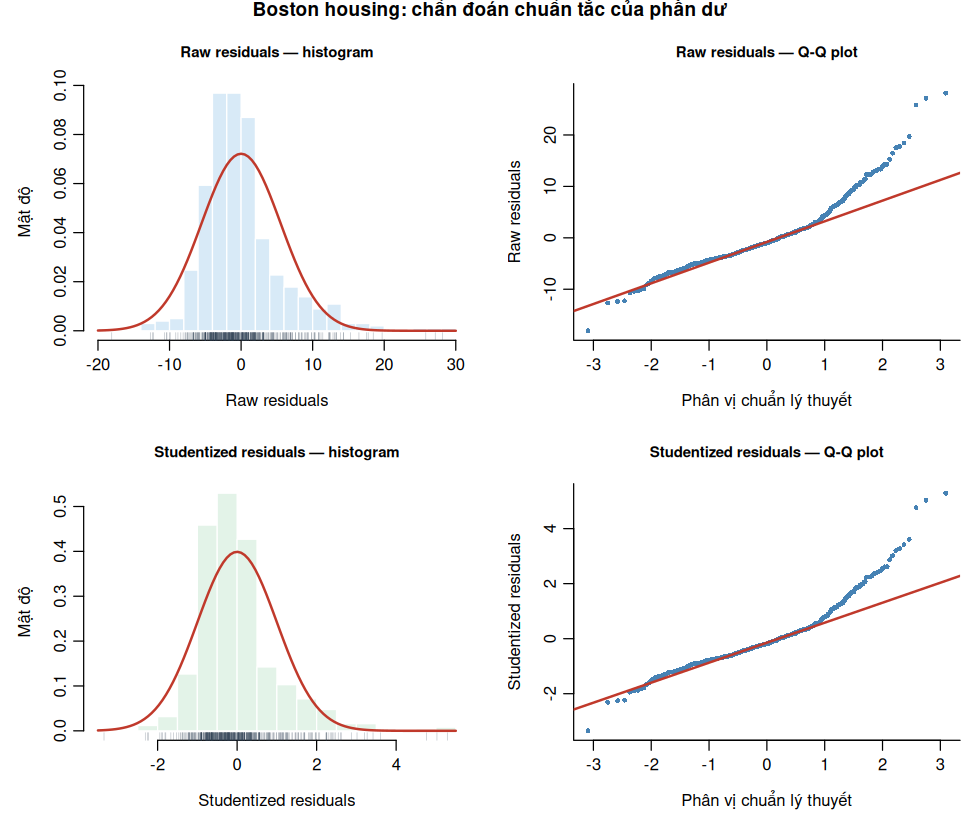
\includegraphics[width=\textwidth,height=0.68\textheight,keepaspectratio]{fig17_boston_normality.png}
  \end{columns}
\end{frame}

% 38
\section{Đồng Nhất Phương Sai}
\begin{frame}{Đồng Nhất Phương Sai: Điều Kiện Toán Học}
  \small
  \[
    \mathrm{Var}(\varepsilon_i\mid \mathbf{x}_i)=\sigma^2
    \qquad \forall i.
  \]
  Dạng ma trận:
  \[
    \mathrm{Var}(\boldsymbol{\varepsilon}\mid\mathbf{X})
    =
    \sigma^2\mathbf{I}.
  \]
  \mathnote{Điều kiện này không nói sai số nhỏ; nó nói độ bất định của sai số ổn định trên toàn miền dự báo.}
\end{frame}

% 39
\begin{frame}{Classical OLS Covariance Khi Homoscedasticity Đúng}
  \small
  \[
    \hat{\boldsymbol{\beta}}-\boldsymbol{\beta}
    =
    (\mathbf{X}^{\top}\mathbf{X})^{-1}\mathbf{X}^{\top}\boldsymbol{\varepsilon}.
  \]
  Nếu $\mathrm{Var}(\boldsymbol{\varepsilon}\mid X)=\sigma^2I$:
  \[
    \mathrm{Var}(\hat{\boldsymbol{\beta}}\mid X)
    =
    \sigma^2(\mathbf{X}^{\top}\mathbf{X})^{-1}.
  \]
  Ước lượng cổ điển:
  \[
    \widehat{\mathrm{Var}}(\hat{\boldsymbol{\beta}})
    =
    s^2(\mathbf{X}^{\top}\mathbf{X})^{-1}.
  \]
\end{frame}

% 40
\begin{frame}{Khi Phương Sai Thay Đổi: Ma Trận \texorpdfstring{$\Omega$}{Omega}}
  \small
  Nếu mỗi quan sát có phương sai riêng:
  \[
    \boldsymbol{\Omega}
    =
    \mathrm{diag}(\sigma_1^2,\dots,\sigma_n^2).
  \]
  Khi đó covariance đúng là:
  \[
    \mathrm{Var}(\hat{\boldsymbol{\beta}}\mid X)
    =
    (X^{\top}X)^{-1}X^{\top}\Omega X(X^{\top}X)^{-1}.
  \]
  \begin{block}{Hậu quả}
    Dùng $s^2(X^{\top}X)^{-1}$ tức là thay nhầm toàn bộ $\Omega$ bằng một hằng số $\sigma^2I$.
  \end{block}
\end{frame}

% 41
\begin{frame}{Breusch-Pagan: Hồi Quy Phụ}
  \small
  Giả thuyết:
  \[
    H_0:\mathrm{Var}(\varepsilon_i\mid x_i)=\sigma^2,
    \qquad
    H_1:\mathrm{Var}(\varepsilon_i\mid x_i) \text{ phụ thuộc } x_i.
  \]
  Quy trình:
  \[
    \hat e_i^2 = \gamma_0 + \gamma_1 z_{i1}+\cdots+\gamma_k z_{ik}+v_i.
  \]
  Thống kê LM:
  \[
    LM=nR^2_{aux}\sim\chi^2(k) \quad \text{dưới }H_0.
  \]
\end{frame}

% 42
\begin{frame}{White Test: Tổng Quát Hơn Breusch-Pagan}
  \small
  Hồi quy phụ kiểu White có thể chứa biến gốc, bình phương và tương tác:
  \[
    \hat e_i^2
    =
    \gamma_0+\sum_j\gamma_jX_{ij}
    +\sum_j\delta_jX_{ij}^2
    +\sum_{j<\ell}\theta_{j\ell}X_{ij}X_{i\ell}+v_i.
  \]
  \[
    W=nR^2_{aux}\sim\chi^2(p).
  \]
  \mathnote{White test linh hoạt hơn nhưng số biến phụ tăng nhanh, dễ hao bậc tự do trong mẫu nhỏ.}
\end{frame}

% 43
\begin{frame}{Sandwich Covariance: Bread - Meat - Bread}
  \small
  \[
    \mathrm{Var}(\hat\beta)
    =
    \underbrace{(X^{\top}X)^{-1}}_{\text{bread}}
    \underbrace{(X^{\top}\Omega X)}_{\text{meat}}
    \underbrace{(X^{\top}X)^{-1}}_{\text{bread}}.
  \]
  \[
    X^{\top}\Omega X
    =
    \sum_{i=1}^{n}\sigma_i^2x_ix_i^{\top}.
  \]
  \begin{block}{Ý tưởng Huber-White}
    Không cần ước lượng chính xác từng $\sigma_i^2$; chỉ cần ước lượng vững toàn bộ phần meat.
  \end{block}
\end{frame}

% 44
\begin{frame}{HC0: Thay \texorpdfstring{$\sigma_i^2$}{sigmai2} Bằng \texorpdfstring{$\hat e_i^2$}{ei2}}
  \small
  \[
    \widehat{X^{\top}\Omega X}_{HC0}
    =
    \sum_{i=1}^{n}\hat e_i^2x_ix_i^{\top}.
  \]
  \[
    \widehat{\mathrm{Var}}_{HC0}(\hat\beta)
    =
    (X^{\top}X)^{-1}
    \left(\sum_{i=1}^{n}\hat e_i^2x_ix_i^{\top}\right)
    (X^{\top}X)^{-1}.
  \]
  \[
    SE_{HC0}(\hat\beta_j)
    =
    \sqrt{\left[\widehat{\mathrm{Var}}_{HC0}(\hat\beta)\right]_{jj}}.
  \]
\end{frame}

% 45
\begin{frame}{Leverage và Vì Sao HC0 Có Thể Quá Lạc Quan}
  \small
  Hat matrix:
  \[
    H=X(X^{\top}X)^{-1}X^{\top},\qquad h_{ii}=H_{ii}.
  \]
  Nếu homoscedasticity đúng:
  \[
    \mathrm{Var}(e_i\mid X)=\sigma^2(1-h_{ii}).
  \]
  Quan sát leverage cao có $h_{ii}$ lớn, nên phần dư quan sát được thường bị co lại.
  \begin{block}{Hệ quả}
    Dùng trực tiếp $\hat e_i^2$ có thể đánh giá thấp meat, đặc biệt trong mẫu nhỏ.
  \end{block}
\end{frame}

% 46
\begin{frame}{HC3: Điều Chỉnh Theo Leverage}
  \small
  MacKinnon-White HC3 dùng:
  \[
    \widehat{\mathrm{Var}}_{HC3}(\hat\beta)
    =
    (X^{\top}X)^{-1}
    \left[
      \sum_{i=1}^{n}
      \frac{\hat e_i^2}{(1-h_{ii})^2}x_ix_i^{\top}
    \right]
    (X^{\top}X)^{-1}.
  \]
  \begin{itemize}
    \item $(1-h_{ii})^{-2}$ phạt mạnh quan sát leverage cao.
    \item HC3 thường bảo thủ hơn HC0.
    \item Hệ số OLS giữ nguyên; chỉ thay covariance matrix.
  \end{itemize}
\end{frame}

% 47
\begin{frame}{Ví Dụ Prestige: Chẩn Đoán Phương Sai}
  \begin{columns}[T,onlytextwidth]
    \column{0.38\textwidth}
      \small
      \begin{itemize}
        \item Mô hình: \texttt{prestige \(\sim\) income + education}.
        \item Breusch-Pagan chưa bác bỏ ở mức 5\%.
        \item White-style test gợi ý cấu trúc phương sai phức tạp hơn.
      \end{itemize}
    \column{0.58\textwidth}
      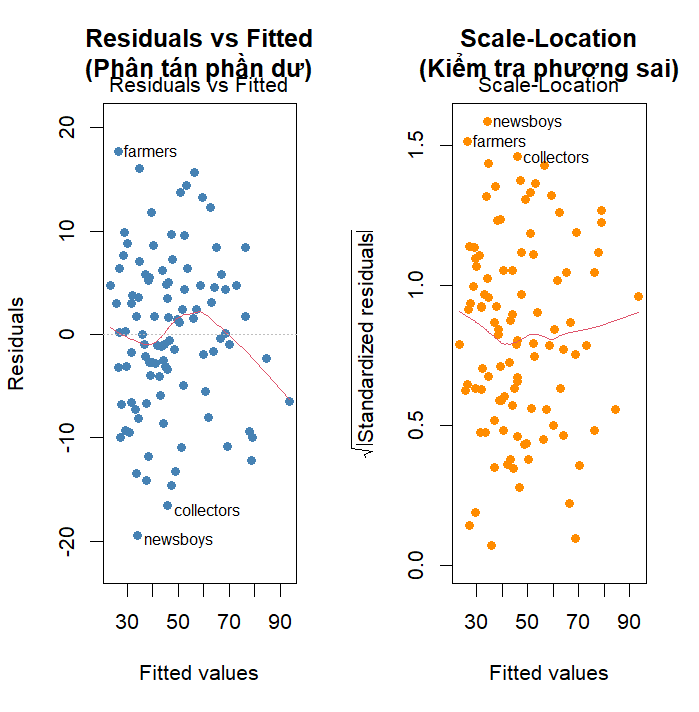
\includegraphics[width=\textwidth,height=0.68\textheight,keepaspectratio]{homoscedasticity_diagnostics.png}
  \end{columns}
\end{frame}

% 48
\begin{frame}{Prestige: HC3 Làm Suy Diễn Thận Trọng Hơn}
  \begin{columns}[T,onlytextwidth]
    \column{0.4\textwidth}
      \small
      \begin{itemize}
        \item HC3 không đổi hệ số OLS.
        \item HC3 điều chỉnh độ bất định của hệ số.
        \item Khoảng tin cậy thường rộng hơn khi SE cổ điển quá lạc quan.
      \end{itemize}
    \column{0.56\textwidth}
      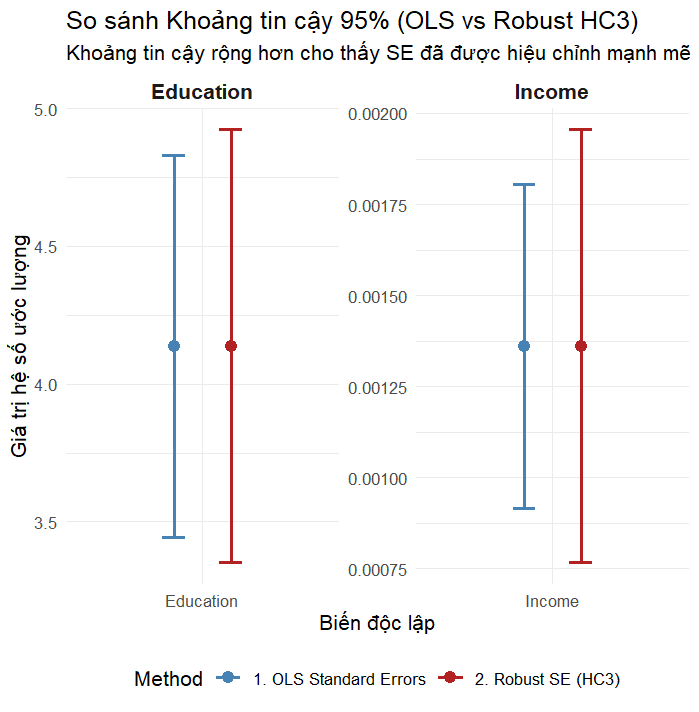
\includegraphics[width=\textwidth,height=0.68\textheight,keepaspectratio]{homoscedasticity_hc3_ci.png}
  \end{columns}
\end{frame}

% 49
\section{Tính Độc Lập Của Sai Số}
\begin{frame}{Tính Độc Lập Của Sai Số: Điều Kiện Ma Trận}
  \small
  Dạng mạnh của giả định là độc lập có điều kiện:
  \[
    \varepsilon_i\perp\!\!\!\perp\varepsilon_j\mid X,
    \qquad i\neq j.
  \]
  Điều kiện bậc hai thường dùng trong Gauss--Markov là:
  \[
    \mathrm{Cov}(\varepsilon_i,\varepsilon_j\mid X)=0,
    \qquad i\neq j.
  \]
  Nếu có tự tương quan:
  \[
    \Omega_{ij}=\mathrm{Cov}(\varepsilon_i,\varepsilon_j\mid X)\neq 0
    \quad\text{cho một số } i\neq j.
  \]
\end{frame}

% 50
\begin{frame}{Sai Số Không Độc Lập Làm Sai Covariance Của OLS}
  \small
  Nếu $E(\varepsilon\mid X)=0$ còn đúng, hệ số OLS có thể vẫn không chệch. Nhưng covariance đúng là:
  \[
    \mathrm{Var}(\hat\beta\mid X)
    =
    (X^{\top}X)^{-1}X^{\top}\Omega X(X^{\top}X)^{-1}.
  \]
  Công thức cổ điển $s^2(X^{\top}X)^{-1}$ bỏ qua các phần tử ngoài đường chéo của $\Omega$.
  \begin{block}{Hậu quả}
    $t$-test, $F$-test, confidence interval và prediction interval có thể không đáng tin.
  \end{block}
\end{frame}

% 51
\begin{frame}{Mô Hình AR(1) Cho Sai Số}
  \small
  Một cấu trúc tự tương quan phổ biến:
  \[
    \varepsilon_t=\rho\varepsilon_{t-1}+u_t,
    \qquad
    u_t\sim (0,\sigma_u^2).
  \]
  Khi $|\rho|<1$:
  \[
    \mathrm{Cov}(\varepsilon_t,\varepsilon_{t-h})
    =
    \frac{\sigma_u^2}{1-\rho^2}\rho^h.
  \]
  \begin{itemize}
    \item $\rho>0$: sai số cùng dấu có xu hướng kéo dài.
    \item $\rho<0$: sai số có xu hướng dao động đổi dấu.
  \end{itemize}
\end{frame}

% 52
\begin{frame}{Nguyên Nhân Làm Sai Số Không Độc Lập}
  \begin{columns}[T,onlytextwidth]
    \column{0.48\textwidth}
      \small
      \begin{itemize}
        \item Dữ liệu có quán tính theo thời gian.
        \item Thiếu biến xu hướng hoặc mùa vụ.
        \item Sai dạng hàm hoặc bỏ sót độ trễ.
        \item Quan sát gần nhau trong không gian có liên hệ.
      \end{itemize}
    \column{0.48\textwidth}
      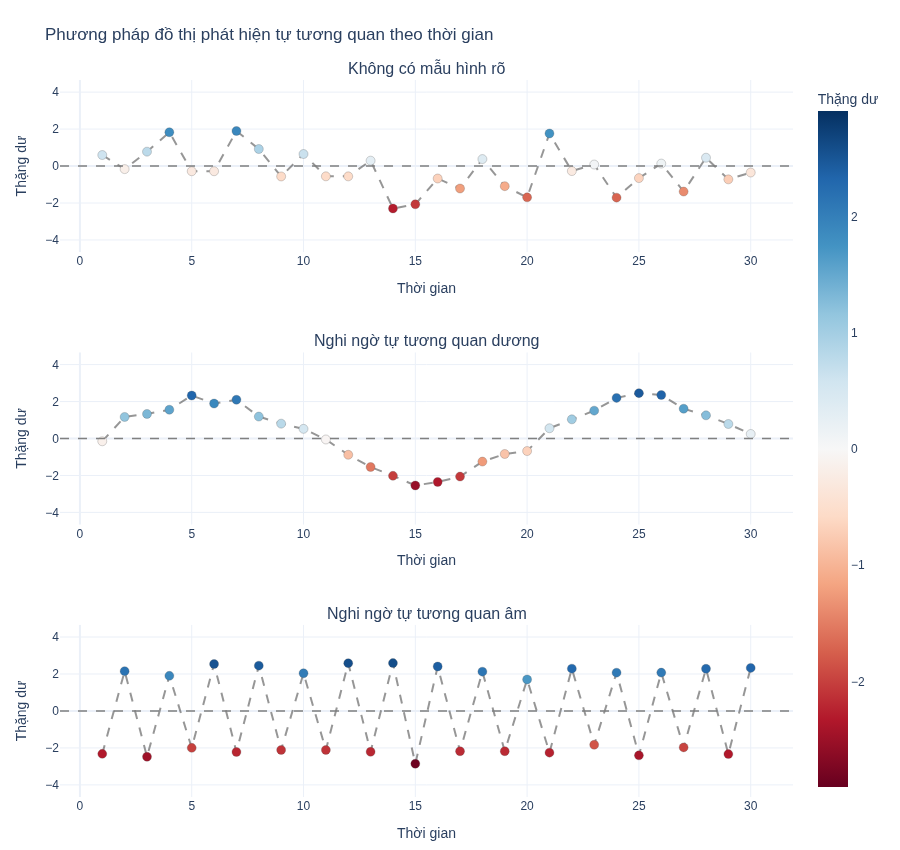
\includegraphics[width=\textwidth,height=0.68\textheight,keepaspectratio]{plot_ts.png}
  \end{columns}
\end{frame}

% 53
\begin{frame}{Durbin-Watson: Công Thức và Diễn Giải}
  \small
  \[
    d
    =
    \frac{\sum_{t=2}^{n}(e_t-e_{t-1})^2}
    {\sum_{t=1}^{n}e_t^2}.
  \]
  Xấp xỉ quan trọng:
  \[
    d\approx 2(1-\hat\rho).
  \]
  \begin{tabularx}{\textwidth}{@{}lX@{}}
    \toprule
    Giá trị $d$ & Diễn giải \\
    \midrule
    $d\approx 2$ & ít bằng chứng tự tương quan bậc 1 \\
    $d<2$ & nghiêng về tự tương quan dương \\
    $d>2$ & nghiêng về tự tương quan âm \\
    \bottomrule
  \end{tabularx}
\end{frame}

% 54
\begin{frame}{Breusch-Godfrey: Kiểm Tra Bậc Cao}
  \small
  Giả sử muốn kiểm tra tự tương quan đến bậc $p$:
  \[
    \varepsilon_t
    =
    \rho_1\varepsilon_{t-1}+\cdots+\rho_p\varepsilon_{t-p}+u_t.
  \]
  Giả thuyết:
  \[
    H_0:\rho_1=\cdots=\rho_p=0.
  \]
  Hồi quy phụ dùng phần dư trễ và biến gốc, rồi tính:
  \[
    LM=nR^2_{aux}\sim\chi^2(p).
  \]
\end{frame}

% 55
\begin{frame}{Chẩn Đoán Bằng Đồ Thị}
  \begin{columns}[T,onlytextwidth]
    \column{0.38\textwidth}
      \small
      \begin{itemize}
        \item Vẽ phần dư theo thời gian hoặc thứ tự quan sát.
        \item Tìm run dài cùng dấu, xu hướng, chu kỳ.
        \item Với dữ liệu không gian, xem phần dư theo vị trí/khu vực.
      \end{itemize}
    \column{0.58\textwidth}
      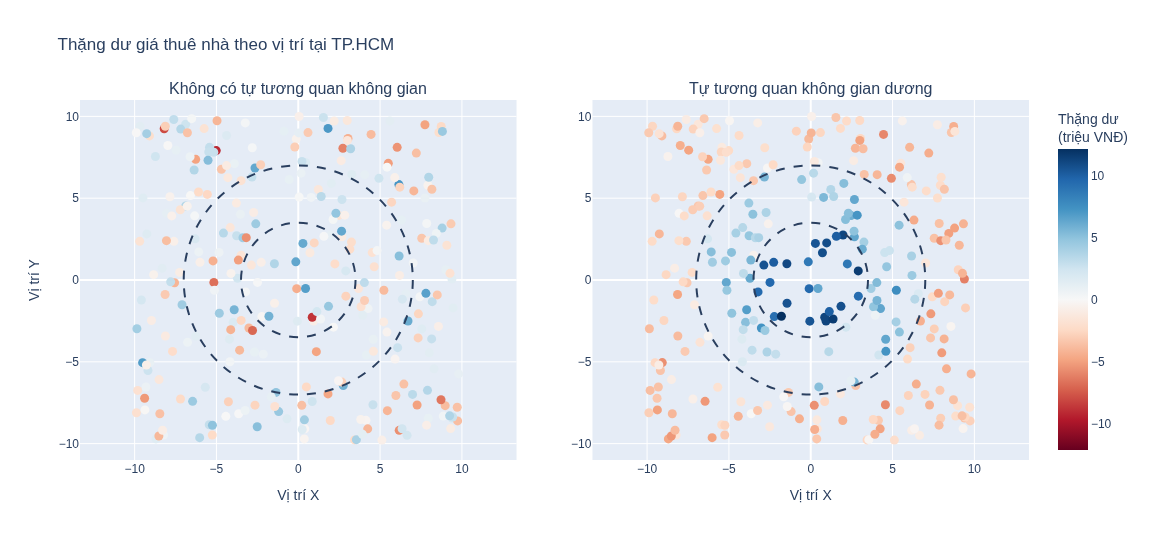
\includegraphics[width=\textwidth,height=0.68\textheight,keepaspectratio]{rent_house.png}
  \end{columns}
\end{frame}

% 56
\begin{frame}{Ví Dụ Doanh Thu: Output Tốt Chưa Đủ}
  \begin{columns}[T,onlytextwidth]
    \column{0.42\textwidth}
      \small
      \begin{itemize}
        \item $R^2$ cao và p-value nhỏ không chứng minh phần dư độc lập.
        \item DW và BG đều có thể bác bỏ $H_0$ sai số độc lập theo nghĩa không tự tương quan.
        \item Cần sửa cấu trúc thời gian hoặc dùng SE phù hợp.
      \end{itemize}
    \column{0.54\textwidth}
      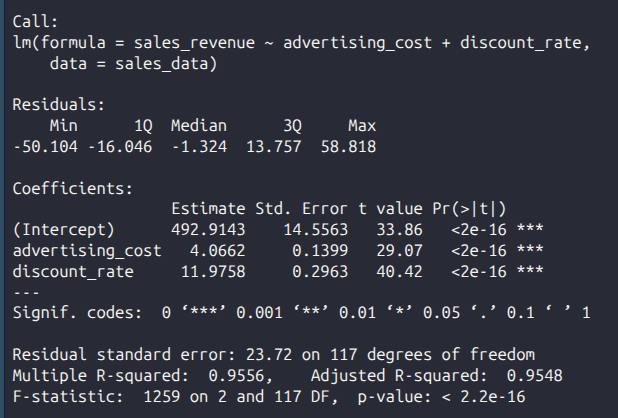
\includegraphics[width=\textwidth,height=0.65\textheight,keepaspectratio]{summary.png}
  \end{columns}
\end{frame}

% 57
\section{Workflow}
\begin{frame}{Workflow Kiểm Tra Giả Định}
  \small
  \begin{enumerate}
    \item Fit OLS và viết rõ dạng $E(Y\mid X)$.
    \item Kiểm tra residuals vs fitted để phát hiện sai dạng hàm.
    \item Kiểm tra Q-Q plot, leverage, Cook's distance nếu suy diễn mẫu nhỏ quan trọng.
    \item Kiểm tra heteroscedasticity bằng Scale-Location, BP/White.
    \item Nếu dữ liệu có thứ tự, kiểm tra autocorrelation bằng residual order plot, DW/BG.
    \item Báo cáo hệ số, SE loại nào, và giả định nào đã được kiểm tra.
  \end{enumerate}
\end{frame}

% 58
\begin{frame}{Bảng Tổng Hợp Toán Học}
  \scriptsize
  \begin{tabularx}{\textwidth}{@{}l>{\raggedright\arraybackslash}X>{\raggedright\arraybackslash}X>{\raggedright\arraybackslash}X@{}}
    \toprule
    Giả định & Điều kiện & Nếu vi phạm & Công cụ \\
    \midrule
    Tuyến tính & $E(Y\mid X)=X\beta$ & Bias hệ số & Residual plot, AV plot, transform/spline \\
    Chuẩn & $\varepsilon\mid X\sim N(0,\sigma^2I)$ & $t/F/\chi^2$ mẫu nhỏ không chính xác & Q-Q, Shapiro, JB, bootstrap \\
    Đồng nhất phương sai & $\Omega=\sigma^2I$ & SE cổ điển sai & BP, White, HC3 \\
    Tính độc lập của sai số & $\varepsilon_i\perp\!\!\!\perp\varepsilon_j\mid X$; $\Omega_{ij}=0$ với $i\neq j$ & SE/test/CI sai theo thứ tự dữ liệu & DW, BG, HAC/GLS \\
    \bottomrule
  \end{tabularx}
\end{frame}

% 59
\begin{frame}{Ba Takeaways Cho Lớp Thạc Sĩ}
  \large
  \begin{enumerate}
    \item OLS là phép chiếu hình học; các giả định quyết định tính chất thống kê của phép chiếu đó.
    \item Normality bảo vệ phân phối kiểm định mẫu nhỏ; homoscedasticity và independence bảo vệ covariance cổ điển.
    \item Khi covariance cổ điển sai, phải nói rõ dùng HC3/HAC/GLS hay sửa mô hình, không chỉ báo cáo p-value mặc định.
  \end{enumerate}
\end{frame}

% 60
\begin{frame}{Tài Liệu Tham Khảo Chính}
  \small
  \begin{itemize}
    \item Weisberg, S. \textit{Applied Linear Regression}.
    \item Rencher, A. C., \& Schaalje, G. B. \textit{Linear Models in Statistics}.
    \item Faraway, J. J. \textit{Linear Models with R}.
    \item Breusch \& Pagan; White; Koenker; MacKinnon \& White.
    \item Gujarati, D. N., \& Porter, D. C. \textit{Basic Econometrics}.
  \end{itemize}
\end{frame}

% 61
\begin{frame}
  \centering
  \Huge Q\&A

  \vspace{0.5cm}
  \large Cảm ơn cô và các bạn đã lắng nghe.
\end{frame}

\end{document}
